\documentclass[titlepage=firstiscover, captions=tableheading, bibliography=totoc]{scrartcl}
\usepackage[autostyle=true,german=quotes]{csquotes}
\usepackage{scrhack}
\usepackage{caption}
\usepackage[aux]{rerunfilecheck}
\usepackage{subcaption}        
\usepackage{fontspec}
\usepackage[dvips]{graphicx}
\usepackage{floatflt,epsfig} 
    
\usepackage{polyglossia}
\setmainlanguage{german}

\usepackage[unicode]{hyperref}
\usepackage{bookmark}
\title{V27\\ Der Helium-Neon-Laser}
\author{
Miriam Simm\\
\texorpdfstring{\href{mailto:miriam.simm@tu-dortmund.de}{miriam.simm@tu-dortmund.de}\and}{,}
Katrin Bolsmann\\
\texorpdfstring{\href{mailto:katrin.bolsmann@tu-dortmund.de}{katrin.bolsmann@tu-dortmund.de}}{}
}
\date{Durchführung: 15.06.2020 \\ Abgabe: -.06.2020}
\usepackage{amsmath} 
\usepackage{amssymb} 
\usepackage{mathtools}
\usepackage[
    math-style=ISO,
    bold-style=ISO,
    sans-style=italic,
    nabla=upright,
    partial=upright,
]{unicode-math}
    
\setmathfont{Latin Modern Math}

\usepackage[
  locale=DE,
  separate-uncertainty=true, 
  per-mode=symbol-or-fraction,
]{siunitx}

\usepackage{multicol}
\setlength{\columnsep}{1pt} %space between columns 

\usepackage{booktabs}
\usepackage[x11names, table]{xcolor}
\usepackage{graphicx}
\usepackage{grffile}
\usepackage{xfrac}
\usepackage{xcolor}

\usepackage{float}
\floatplacement{figure}{h}
\floatplacement{table}{h}
\usepackage[
  section,
  below,
]{placeins}

\usepackage{expl3}
\usepackage{xparse}
\ExplSyntaxOn
\NewDocumentCommand \E {} {\symup{e}}
\ExplSyntaxOff

% Literaturverzeichnis
\usepackage[
  backend=biber,
]{biblatex}
% Quellendatenbank
\addbibresource{literatur.bib}

\usepackage[
  version=4,
  math-greek=default,
  text-greek=default,
]{mhchem}
 

\raggedcolumns

\begin{document}

\maketitle
\section{Zielsetzung}
Ziel dieses Versuches ist die Untersuchung der Spektren von unbekannten Strahlern bezüglich der Energie und Aktivität.
Hierzu werden zuerst die Detektoreigenschaften anhand bekannter Strahler bestimmt. 

\section{Theorie}
\subsection{Wechselwirkung von Gamma-Strahlung mit Materie}
Durch Wechselwirkung mit Materie wird die Ausbreitungsrichtung der Gamma-Quanten geändert oder diese werden annihiliert, sodass die Intensität gemäß des Lambert-Beerschen-Gesetzes
\begin{equation}
I(x) = I_0 \exp(-\mu x)
\end{equation}
abnimmt.
Wobei $I_0$ der ursprünglichen Intensität und $x$ der zurückgelegten Strecke im Medium entspricht.
Die mittlere Reichweite der Gamma-Strahlung in diesem Medium entspricht dem Kehrwert des Extinktionskoeffizienten, welcher sich mit der Ordnungszahl $Z$, der Teilchenzahldichte $n$ und dem Wirkungsquerschnitt $\sigma$ gemäß der Formel
\begin{equation}\label{eq:mu}
\mu = Zn\sigma
\end{equation}
beschreiben lässt.

\FloatBarrier
\begin{figure}[h]
\begin{minipage}[t]{0.48\textwidth}
\vspace{0pt}
Der Wirkungsquerschnitt setzt sich wiederum aus verschiedenen Wechselwirkungen zusammen, welche je nach Energie verschieden starke Beiträge liefern.
So dominiert bei geringeren Energien der Photoeffekt, während bei hohen Energien die Paarbildung den größen Beitrag des Wirkungsquerschnittes liefert.
Der Comptoneffekt ist bei fast allen Energien präsent, liefert jedoch nur für Energien zwischen $100\, \si{\keV}$ und $10\,\si{\MeV}$ einen relevanten Beitrag.
In Abbildung \ref{fig:tfig1} ist der Verlauf des Extinktionskoeffizient $\mu$ zu sehen.
Da es sich bei den in Abbildung \ref{fig:tfig1} beschriebenen Prozessen um die drei wichtigsten Prozesse bezogen auf Absorption von Gamma-Strahlung in Materie handelt, sollen diese im Folgenden genauer erläutert werden.
\end{minipage}
\hfill
\begin{minipage}[t]{0.50\textwidth}
\vspace{-10pt}
\centering
\includegraphics[width=\textwidth]{Absorption.png}
\caption{Der Extinktionskoeffizient in Abhängigkeit der Energie für verschiedene Wechselwirkungsprozesse: Photoeffekt, Comptoneffekt und Paarbildung \cite{quelle02}.}
\label{fig:tfig1}
\end{minipage}
\end{figure}
\FloatBarrier

\subsubsection*{Der Photoeffekt}
Der Photoeffekt beschreibt die Wechselwirkung einen Gamma-Quants mit einem Hüllenelektron, welches vorzugsweise aus der K-Schale stammt.
Bei diesem Prozess absorbiert das Elektron die gesamte Energie des Photons, sodass dieses annihiliert wird.
\FloatBarrier
\begin{figure}[h]
\begin{minipage}[t]{0.4\textwidth}
\vspace{0pt}
\centering
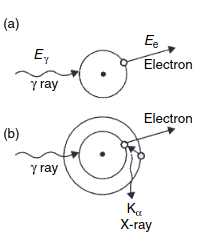
\includegraphics[width=1.1\textwidth]{Photoeffekt.png}
\caption{Der Photoeffekt ohne (a) und mit (b) Emission eines Photons \cite{quelle02}.}
\label{fig:tfig2}
\end{minipage}
\hfill
\begin{minipage}[t]{0.58\textwidth}
\vspace{0pt}
Unter der Vorraussetzung, dass die Energie des Photons größer ist als die Bindungsenergie des Elektrons, wird dieses aus der Elektronenhülle gelöst.
Die restliche Energie wird dem Elektron als kinetische Energie übertragen.
Das vom Elektron hinterlassene Loch in der Elektronenschale, wird durch eine Kaskade an Elektronenübergängen erneut besetzt.
Bei diesem Prozess besetzen nacheinander Elektron aus höherenergetischen Schalen das Loch der nächst tieferen Schale und hinterlassen somit wiederum ein Loch.
Jeder dieser Übergangsprozesse emittiert ein Photon, welches genau der Energiedifferenz der beiden Schalen entspricht und somit dem Spektrum der Röntgenstrahlung zugeordnet wird.
Aufgrund der geringen Reichweite der Röntgenstrahlung, kann angenommen werden, dass durch den Photoeffekt die gesamte Energie des Photons im Detektor verbleibt und detektiert werden kann.
\end{minipage}
\end{figure}
\FloatBarrier

Unter der Annahme, dass die Photonenenergie im Bereich des Photoeffektes größer als die Bindungsenergie des Elektrons aber klein gegenüber der Elektronenmasse $m_ec^2$ ist, ist eine nichtrelativistische Näherung gerechtfertigt.
Außerdem wird von der Born'schen Näherung ausgegangen, welche eine ebene Welle für das freigesetzt Elektron annimmt.
Somit kann der Wirkungsquerschnitt des Photoeffektes näherungsweise durch die Formel \cite{quelle03}
\begin{equation}
\sigma_{\text{Ph}}=\sqrt{32}\alpha^4 \epsilon^\frac{7}{2}Z^5\sigma_{Th}\, , \qquad \epsilon = \frac{E_{\gamma}}{m_e c^2}
\end{equation}
beschrieben werden.
Hierbei ist $\alpha = \frac{1}{137}$ die Feinstrukturkonstante und $\sigma_{\text{Th}}=\frac{8}{3}\pi r_e^2$ der Thomson-Wirkungsquerschnitt mit dem klassischen Elektronenradius $r_e$.

\subsubsection*{Der Comptoneffekt}
Als Comptoneffekt wird die Streuung eines Photons an einem freien Elektron oder an einem quasifreien Hüllenelektron bezeichnet.
Aus Energie- und Impulserhaltung errechnet sich für die Energie des gestreuten Photons in Abhängigkeit des Streuwinkels der Zusammenhang
\begin{equation}
E'_{\gamma} = \frac{E_{\gamma}}{1 + \epsilon(1-\cos(\theta))} \, .
\end{equation}
Somit ergibt sich für einen Streuwinkel von $\theta = 180°$ der maximale Energieübertrag von
\begin{equation}
\Delta E_\text{max} = \frac{2\epsilon}{1 + 2 \epsilon} E_{\gamma} \, .
\end{equation}
Offensichtlich kann das Photon durch die Comptonwechselwirkung nicht seine gesamte Energie auf das Elektron übertragen, sodass das es bei diesem Prozess nicht annihiliert wird.
Somit ist das Energiespektrum der gestreuten Elektronen kontinuierlich und wird auch Comptonkontinuum genannt. 
Bei der Maximalenergie, welche für $\theta = 180°$ übertragen wird, bricht dieses abrupt ab und bildet die Comptonkante.
Der Comptoneffekt ist schematisch in Abbildung \ref{fig:tfig4} dargestellt.

\begin{figure}
\centering
\begin{subfigure}{0.55\textwidth}
\centering
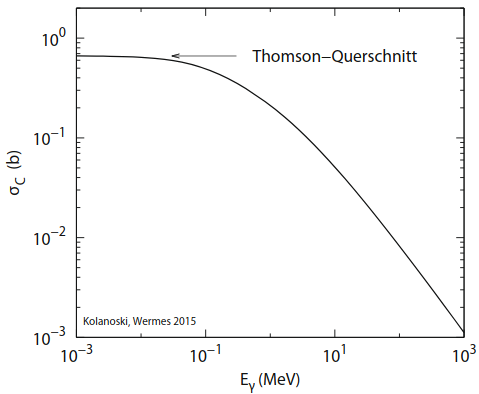
\includegraphics[width=1.03\textwidth]{compton2.png}
\captionsetup{format=hang, labelfont = bf, textfont = small}
\caption{Comptonwirkungsquerschnitt pro Hüllenelektron gegen die Energie des Photons aufgetragen \cite{quelle03}.}
\label{fig:tfig3}
\end{subfigure}
\begin{subfigure}{0.42\textwidth}
\vspace{35pt}
\centering
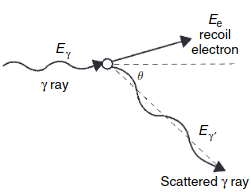
\includegraphics[width=0.9\textwidth]{Compton.png}
\vspace{39pt}
\captionsetup{format=hang, labelfont = bf, textfont = small}
\caption{Schematische Darstellung des Comptoneffekts \cite{quelle02}.}
\label{fig:tfig4}
\end{subfigure}
\caption{Schematische Darstellung der Kinematik des Comptoneffekts, sowie der Energieabhängigkeit des Wirkungsquerschnittes pro Hüllenelektron.}
\vspace{15pt}
\label{fig:tfig34}
\end{figure}
\noindent
Der differentielle Wirkungsquerschnitt wird durch die Klein-Nishina-Formel
\begin{equation}
\frac{d \sigma_C}{dE} = \frac{3}{8}\frac{\sigma_{\text{Thomson}}}{m_e c^2 \epsilon^2}\left(2+\left(\frac{E}{E_{\gamma}-E}\right)^2
\left(\frac{1}{\epsilon^2}+\frac{E_{\gamma}-E}{E_{\gamma}}-\frac{2}{\epsilon}\frac{E_{\gamma}-E}{E_{\gamma}}\right)\right)
\end{equation}
beschrieben.
Durch Integration ergibt sich für den totalen Wirkungsquerschnitt pro Elektron \cite{quelle03}
\begin{equation}
\sigma_C = 2\pi r_e^2\left[\frac{1+\epsilon}{\epsilon^2}\left(\frac{2(1+\epsilon)}{1+2\epsilon}-\frac{1}{\epsilon}\ln(1+2\epsilon)\right)
+\frac{1}{2\epsilon}\ln(1+2\epsilon)-\frac{1+3\epsilon}{(1+2\epsilon)^2}\right]\, .
\end{equation}
Somit gilt für den totalen Wirkungsquerschnitt eines Atoms der Kernladungszahl $Z$ der Zusammenhang
\begin{equation}
\sigma_C^{\text{Atom}} = Z \sigma_C \sim \frac{Z}{E_{\gamma}}\, .
\end{equation}
In Abbildung \ref{fig:tfig3} ist der Verlauf des Comptonwirkungsquerschnittes in Abhängigkeit von der Photonenenergie zu sehen.

\subsubsection*{Die Paarerzeugung}\label{sec:paar}
Ist die Photonenenergie größer als die doppelte Ruhenergie eines Elektrons kommt es zur Erzeugung eines Elektron-Positron-Paares.
Hierbei wird die gesamte Energie des Photons in die Ruheenergie des Elektrons und Positrons, sowie dessen kinetische Energien umgewandelt.
Damit der Impuls erhalten bleibt, bedarf es einen weiteren Stoßpartner, bei dem es sich meistens um einen Atomkern des Absorbermaterials handelt.

Das Positron annihiliert kurz nach seiner Entstehung mit einem, im Detektor vorhandenen Elektron, sodass zwei Photonen entstehen.
Die Gesamtenergie des Photons verbleibt nur dann vollständig im Detektor, wenn diese beiden Photonen und Elektron ebenso dort verbleiben.
Es besteht jedoch eine endliche Wahrscheinlichkeit dass ein Teil der Energie aus dem Detektor entweicht.
Entweicht eins von den beiden Photonen, wird von einem Single escape gesprochen, Entweichung beider Photonen, wird dementsprechend Double excape genannt.

Der Wirkungsquerschnitt ist davon abhängig, wie stark der Atomkern von den Elektronenhüllen abgeschirmt wird, daher werden zwei Fälle unterschieden:
\begin{align}
\intertext{$\qquad\bullet$ geringe Abschirmung: } \sigma_{\text{Paar}}&=4Z^2 \alpha r_e^2 \left(\frac{7}{9}\ln(2\epsilon)-\frac{109}{54}\right)\\
\intertext{$\qquad\bullet$ vollständige Abschirmung: } \sigma_{\text{Paar}}&=4Z^2 \alpha r_e^2 \left(\frac{7}{9}\ln(\frac{183}{Z^{1/3}})-\frac{1}{54}\right)
\end{align}
Im Falle vollständiger Abschirmung ist der Wirkungsquerschnitt unabhängig von der Energie des Photons.
Für den Fall geringer Abschirmung ergibt sich ein differentieller Wirkungsquerschnitt von
\begin{equation}
\frac{d\sigma}{d E} = \frac{28\alpha Z² r_e^2}{9E_{\gamma}}\, .
\end{equation}

Abbildung \ref{fig:tfig5} bietet einen Überblick über die drei beschriebenen Wechselwirkungsprozesse der Gamma-Quanten im Detektor.

\FloatBarrier
\begin{figure}
\centering
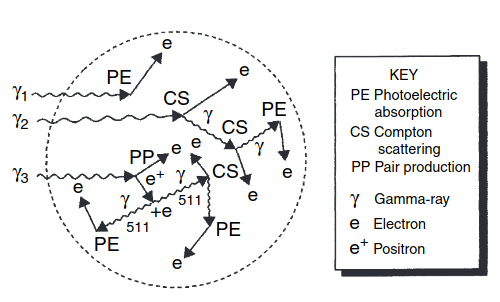
\includegraphics[height=6cm]{alles.png}
\caption{Übersicht der wichtigsten Absorptionsprozesse im Detektor \cite{quelle02}.}
\label{fig:tfig5}
\end{figure}
\FloatBarrier

\subsection{Grundlagen der Halbleiterinstrumente}
Der Germanium Detektor macht sich einige grundlegende Eigenschaften von dotierten Halbleitern zu nutze, welche im Folgenden genauer erläutert werden sollen.

Germanium besitzt 4 Valenzelektronen pro Atom, sodass durch das Einbringen eines Fremdatoms, welches auch Donatoratom genannt wird, mit 5 Valenzatomen, eins der Elektronen sich quasifrei bewegen kann und als Ladungsträger dient.
In diesem Fall wird von n-Dotierung gesprochen.
Somit dominieren in einem n-dotierten Halbleiter die Elektronen als Ladungsträger und die Fermienergie liegt nahe am Leitungsband.
Wird stattdessen ein Fremdatom mit 3 Valenzelektronen in das Germanium eingebracht, so entsteht ein Loch, welches als positiver Ladungsträger zur Verfügung steht.
Aufgrund der Eigenschaft des Fremdatoms, ein weiteres Elektron binden zu können, werden diese auch Akzeptoren genannt und in diesem Fall liegt ein p-dotierter Halbleiter vor.
In einem p-dotierten Halbleitern dienen also hauptsächlich Löcher als Ladungsträger und die Fermienergie liegt nahe am Valenzband.

\FloatBarrier
\begin{figure}[h]
\begin{minipage}[t]{0.45\textwidth}
\vspace{10pt}
\centering
\includegraphics[width = 1.05\textwidth]{pnübergang.png}
\caption{Drift und Diffusionstrom an einer pn-Grenzschicht \cite{quelle03}.}
\label{fig:tfig6}
\end{minipage}
\hfill
\begin{minipage}[t]{0.53\textwidth}
\vspace{0pt}
Grenzen p- und n-dotierte Halbleiter direkt aneinander entsteht ein pn-Übergang, wie in Abbildung \ref{fig:tfig6} gezeigt ist.
Aufgrund des Konzentrationsgefälles am pn-Übergang kommt es zu einem Diffusionsstrom, sodass die Donatorelektronen der n-dotierten Seite auf die p-dotierte Seite diffundieren und die Löcher der p-dotierten Seite auf die n-dotierte Seite.
Somit kommt es zu einer Rekombination der Ladungsträger und es bildet sich eine Verarmungszone, in welcher kaum freie Ladungsträger vorhanden sind und die Leitfähigkeit erheblich abnimmt.
Aufgrund der ionisierten Atomrümpfe entsteht eine positive Ladungsdichte an der n-Grenzschicht und eine negative Ladungsdichte an der p-Grenzschicht, sodass sich ein elektrisches Feld ausbildet.
Dieses Feld wirkt wiederum dem Diffusionstrom entgegen, sodass sich ein Gleichgewichtszustand einstellt, in welchem die Verarmungszone eine endliche Breite $d$ besitzt.
\end{minipage}
\end{figure}
\FloatBarrier
Im Allgemeinen ist die Verarmungszone sehr schmal. 
Die Breite kann jedoch durch das Anlegen einer äußeren Spannung vergrößert werden. 
Dies ist essentiell für das hohe Energieauflösevermögen des Germaniumdetektors und wird im folgenden Abschnitt genauer erörtert.

\subsection{Der Halbleiter Detektor}
In diesem Versuch wird als Detektor ein koaxialer Germanium-Detektor verwendet, welcher in Abbildung \ref{fig:tfig7} zu sehen ist.
Dieser befindet sich unter einer Aluminium-Schutzhaube, sodass die einfallenden Gamma-Quanten mindestens eine Energie von $40-50\,\si{keV}$ besitzen müssen, um diese und die erste Schichte des Detektors überwinden zu können.
Die Oberfläche des Detektors ist mit Lithium-Atomen n-dotiert und besitzt somit eine hohe Leitfähigkeit.
Im Inneren befindet sich eine Bohrung, dessen Oberfläche mit Gold-Atomen p-dotiert ist.
Beide dotierten Schichten dienen zum Anschluss einer äußeren Spannung.
Diese wird so angelegt dass die n-dotierte Schicht für den Anschluss des Pluspols dient.
Durch die angelegte Spannung bildet sich eine ausgedehnte Verarmungszone innerhalb des Detektors, welche den Detektorbereich bildet.

\FloatBarrier
\begin{figure}
\centering
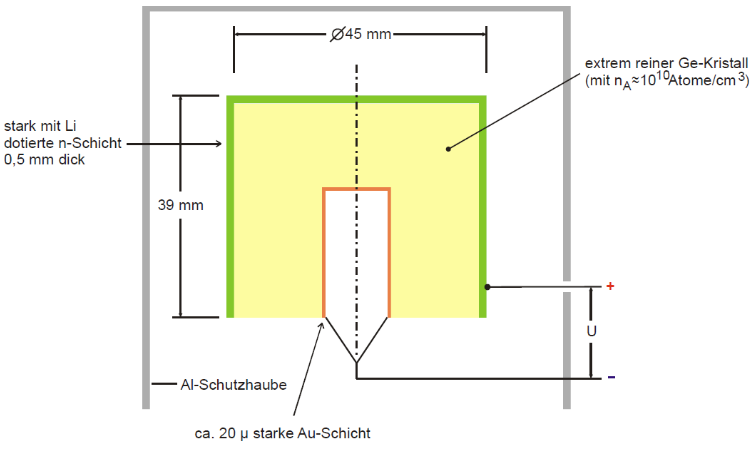
\includegraphics[width = 0.9\textwidth]{Detektor.png}
\caption{Querschnitt des koaxialen Germaniumdetektors, sowie dessen Maße \cite{quelle01}.}
\label{fig:tfig7}
\end{figure}
\FloatBarrier

Der gesamte Aufbau, wie er in Abbildung \ref{fig:tfig7} zu sehen ist, befindet sich in einem Bleigehäuse, welches von innen mit Kupferplatten belegt ist.
Dieses dient zur Abschirmung äußerer Strahlung.

Dringt nun ein Gamma-quant von außen in das Gehäuse ein und gelangt in die Veramungszone, finden Wechselwirkungsprozesse mit der Materie statt.
Dabei kommt es unter anderem zum Freisetzen von Elektronen, welche wiederum mit anderen Elektronen zusammenstoßen und somit Elektronen-Loch-Paare erzeugt werden.
Durch die angelegte Spannung werden die Elektron-Loch-Paare voneinander getrennt, bevor sie rekombinieren können.
Somit entsteht ein Ladungsimpuls, welcher verstärkt wird und ein Detektorsignal bildet.
Das Detektorsignal ist proportional zu der deponierten Photonenenergie, denn je mehr Energie von den Photonen auf die Elektronen übertragen wird, desto mehr Elektron-Loch-Paare können erzeugt werden.
Die Elektronen der Paare können ebenfalls Elektron-Loch-Paare erzeugen, sodass eine Kaskade entsteht, die je nach Photonenenergie unterschiedlich stark ausgeprägt ist.

Eine charakteristische Größe des Detektors ist das Auflösungsvermögen, welches durch die Halbwertsbreite $\Delta E_{1/2}$ der Impulshöhenverteilung beschrieben wird.
Das bedeutet, dass zwei Detektorsignale verschiedener Energien $E_1$ und $E_2$ genau dann unterschieden werden können, wenn sie sich mindesten um $\Delta E_{1/2}$ unterscheiden.

Eine weitere Charakteristik eines Detektors ist die Nachweiswahrscheinlichkeit, welche von der Energie abhängig ist.
Diese besagt, wie viele der in den Detektor eingedrungenen Photonen von diesem registriert werden und wird durch die Formel
\begin{equation}
Q=\frac{4\pi}{\Omega}\frac{N}{AW}
\end{equation}
beschrieben.
Hierbei ist $\Omega$ der Raumwinkel, den die Strahlungsquelle vom Detektor abdeckt.
$A$ ist die Aktivität des Strahlers, $W$ die energieabhängige Emissionswahrscheinlichkeit des Strahlers und $N$ entspricht der Zählrate der Gamma-Quanten des Detektors.

\subsection{Das Energiespektrum eines monochromatischen Gammastrahlers}
\FloatBarrier
\begin{figure}
\centering
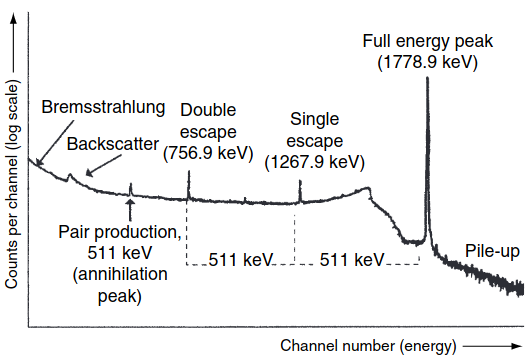
\includegraphics[width = 0.6\textwidth]{Spektrum.png}
\caption{Das Energiespektrum am Beispiel von $^{28}\symup{Al}$. Kurz vor dem Photopeak ist deutlich die Comptonkante zu erkennen. Die Double und Single escape Peaks können der Paarerzeugung zugeordnet werden \cite{quelle02}.}
\label{fig:tfig8}
\end{figure}
\FloatBarrier
Das Energiespektrum eines monochromatischen Gammastrahlers weist einige Charakteristika auf, welche in Abbildung \ref{fig:tfig8} zu sehen sind.
Wesentliche Bestandteile sind das Comptonkontinuum, der Rückstreupeak und der Photopeak.
Der Photopeak wird auch Vollenergiepeak genannt, da er durch den Photoeffekt entsteht, bei welchem die Photonen ihre gesamte Energie im Detektor deponieren.
Das Maximum des Photopeaks entspricht also der Energie der Gammastrahlung.

Das Comptonkontinuum und die Comptonkante entstehen durch die Comptonstreuung.
Die Comptonkante entspricht dabei der Energie, welche bei bei einem Winkel von $180°$ übertragen wird, also dem maximalen Energieübertrag, welcher beim Comptoneffekt auftreten kann.
Da das Photon durch die Comptonstreuung nicht annihiliert wird kommt es auch zu Mehrfachstreuungen, sodass die deponierte Energie teilweise auch größer als die der Comtonkante sein kann.
Aus diesem Grund ist die Comptonkante keine scharfe Kante, sondern ist leicht verschmiert.

Bei einige Gamma-Quanten kommt es auch zu Wechselwirkungen mit der Abschirmung des Detektors und somit zu Energieverlust.
Diese können von der Abschirmung zurückgestreut werden, sodass sie den Detektor mit geringerer Energie erreichen.
Der sich dadurch ergebene Peak wird Rückstreupeak genannt und entspricht einer Energie von
\begin{equation}
E_\text{Rück}= \frac{E_{\gamma}}{1+2\epsilon}\, .
\end{equation}

Die Double und Single escape Peaks entstehen durch die Paarerzeugung.
Eine Erläuterung zu diesem Prozess ist in Abschnitt \ref{sec:paar} zu finden. 

\section{Durchführung}
Zu Beginn der Messung wird eine kalibrierte $^{152}\symup{Eu}$-Probe vermessen, sodass diese zur Energiekalibrierung genutzt werden kann.
Anschließend wird das Spektrum eines $^{137}\symup{Cs}$-Strahlers aufgenommen, sowie das einer $^{133}$-Barium-Quelle.
Zuletzt wird das Spektrum eines unbekannten Strahlers (Bananenchips) vermessen.

\nocite{wingate}
\nocite{*}
\printbibliography
\end{document}
